\chapter{CSS Selector}

\section{What is CSS}

CSS是一种用来指定文档怎么呈现给用户的语言.

文档是一系列使用标记语言组织的信息.

呈现文档的意思是将文档转化为一种对观众有用的格式.

\begin{HTML5}[demo]
<!DOCTYPE html>
<html>
  <head>
  <meta charset="UTF-8">
  <title>Sample document</title>
  </head>

  <body>
    <p>
      <strong>C</strong>ascading
      <strong>S</strong>tyle
      <strong>S</strong>heets
    </p>
  </body>
</html>
\end{HTML5}

\section{Why use CSS}

使得样式和HTML分离
\begin{itemize}
\item 避免重复
\item 更容易维护
\item 在一个地方就可以改变整个网站的样式
\end{itemize}

\begin{CSS}[style1.css]
strong {color:red;}
\end{CSS}

\begin{HTML5}
<!DOCTYPE html>
<html>
  <head>
  <meta charset="UTF-8">
  <title>Sample document</title>
  <link rel="stylesheet" type="text/css" href="style1.css">
  </head>

  <body>
    <p>
      <strong>C</strong>ascading
      <strong>S</strong>tyle
      <strong>S</strong>heets
    </p>
  </body>
</html>
\end{HTML5}

\section{How CSS works}

\begin{itemize}
\item 浏览器将标记语言和CSS转换为DOM.
\item 浏览器展现DOM的内容
\end{itemize}

\section{CSS Rule}

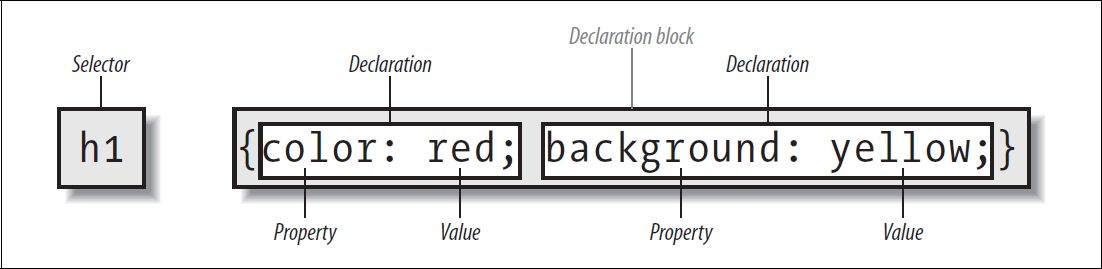
\includegraphics[scale=0.75]{css/resources/css-rule.jpg}

\section{Selector}

The term selector can refer to a simple selector, compound selector, complex selector, or selector list.

A selector list is a comma-separated list of selectors; see Selector Lists.

A complex selector is a chain of one or more compound selectors separated by combinators.

A compound selector is a chain of simple selectors that are not separated by a combinator. It always begins with a type selector or a (possibly implied) universal selector. No other type selector or universal selector is allowed in the sequence.

A simple selector is either a type selector, universal selector, attribute selector, class selector, ID selector, or pseudo-class.

A combinator is punctuation that represents a particular kind of relationship between the compound selectors on either side. Combinators in Selectors level 4 include: whitespace, "greater-than sign" (U+003E, >), "plus sign" (U+002B, +) and "tilde" (U+007E, ~). White space may appear between a combinator and the simple selectors around it.

An empty selector, containing no compound selector, is an invalid selector.


中文版,因为说得不太清楚,所以保留英文版:

select可以是一个simple selector, compound selector, complex selector,或者selector list。

\begin{itemize}

\item simple selector. 就是一个 type selector, universal selector, attribute selector, class selector, ID selector, 或者 pseudo-class.

\begin{CSS}
p { color: red; } /* type selector 选择p元素 */

/* :开头的虚类 */

/* ::开头的虚元素 */

\end{CSS}

\item compound selector, 就是一系列没有被combinator分隔开的simple selector.一般以type selector或者universal selector开头,而且不能再有其他的type selector或者universal selector出现在后面了。

\begin{CSS}

/* 补充代码 */

\end{CSS}

\item complex selector, 一个或者多个compound selector,由combinator分开。 combinator有空格, 大于号 (U+003E, >), 加号 (U+002B, +) 和波浪号 (U+007E, ~)

\begin{CSS}

/* 补充代码*/

\end{CSS}

\item selector list, 通过逗号分隔开的complex selector.

\begin{CSS}

/* 通过逗号分割开的selector。表示对每种selector选择的元素应用样式 */
h1, h2, h3 {color:blue; font-weight:bold;}

/* 补充代码说明 */

\end{CSS}

\end{itemize}


\subsection{Subject of a Selector}

selector从DOM树上选取的元素就是subject of a selector. 默认情况下,subject是由selector的最后一个compound selector表示的元素。 因为combinator引入的是附加的限制,所以subject of a selector是他最后一个compund selector表示的元素的子集。

\begin{CSS}
/* 补充代码 */
\end{CSS}

感叹号改变subject of a selector

\begin{CSS}
/* 补充代码 */
\end{CSS}

\subsection{Selector List}

当多个selector共享同一个declaration时,他们能够被组合成一个使用逗号分开的列表

\begin{CSS}
h1 { font-family: sans-serif }
h2 { font-family: sans-serif }
h3 { font-family: sans-serif }
\end{CSS}

等价于

\begin{CSS}

h1, h2, h3 { font-family: sans-serif }

\end{CSS}


唯一不同的是,当其中有一个selector不生效的时候,上面那种情况只有一条规则不会生效,而后面那种情况,整个这一条规则都将不生效.

\begin{CSS}

h1 { font-family: sans-serif }
h2..foo { font-family: sans-serif } /* 只有这一条不生效, 其他两条是生效的 */
h3 { font-family: sans-serif }


/* 上面不等价于下面 */

h1, h2..foo, h3 { font-family: sans-serif } /* 整条CSS不生效了 */


\end{CSS}


\subsection{Simple selector}



\subsubsection{Type selector}

A type selector is the name of a document language element type.

就是HTML的标签名来选择元素。

\begin{CSS}

/* 补充代码 */

\end{CSS}


\subsubsection{Universal Selector}

* asterisk (* U+002A),用来匹配文档中任何一个标签.


\begin{CSS}

/* 补充代码 */

\end{CSS}

\subsubsection{Attribute Selector}



\subsection{Pseudo-Class \& Pseudo-Element}

\subsubsection{Pseudo-classes}

pseudo-class 用来表示通过dom tree之外的信息来选择,或者其他simple selector来表示的选择。通常是使用单个冒号(:)加上pseudo-class的名字。


\begin{itemize}
\item Pseudo-classes可以在任何compund selector中出现. 
\item Pseudo-classes可以在compund selector的任意位置出现(第一个type selector或者universal selector之后)
\item pseudo-classes大小写敏感,一些相互排斥,一些可以同时使用。
\item Pseudo-classes是动态,可能随着用户的操作,一个元素可能失去或者获得某个Pseudo-classe
\end{itemize}

\paragraph{The hyperlink pseudo-class}

\begin{CSS}

/*匹配作为超链接的元素。 <a>, <area>, or <link> elements with an href */ 
:any-link { ... } 

/* 等价于 */
:matches(:link, :visited) { ... }

\end{CSS}


\paragraph{The link history pseudo-classes}

\begin{itemize}
\item \lstinline$:link$表示没有被访问过的超链接
\item \lstinline$:visited$表示被访问过的超链接

\end{itemize}

\begin{CSS}

/* 补充代码 */



\end{CSS}

\paragraph{The local link pseudo-class}

\lstinline$:local-link$ 基于当前页面的匹配

\begin{CSS}
/*
given the links:
*/

<a href="http://www.example.com">Home</a>
<a href="http://www.example.com/2011">2011</a>
<a href="http://www.example.com/2011/03">March</a>
<a href="http://www.example.com/2011/03/">March</a>
<a href="http://www.example.com/2011/03/21">21 March</a>
<a href="https://www.example.com/2011/03/">March</a>
<a href="http://example.com/2011/03">March</a>

/*
and the styles:
*/

a:local-link {...}
a:local-link(0) {...}
a:local-link(1) {...}
a:local-link(2) {...}
a:local-link(3) {...}

/*
If the document's URL is http://www.example.com/2011/03/:

Link 1 would receive Style B
Link 2 would receive Styles B and C
Link 3 would receive Styles B, C, and D
Link 4 would also receive Styles A, B, C, and D
Link 5 would receive Styles B, C, and D
Link 6 would receive Styles B, C, and D
Link 7 would remain unstyled
Style E would not be applied to anything
*/
\end{CSS}


\paragraph{User Action Pseudo-classes}

\begin{itemize}
\item :link 		/* unvisited links */
\item :visited 		/* visited links */
\item :hover		/* user hovers */
\item :active		/* active links */
\end{itemize}


:target


:lang




%\paragraph{:first-child}

%\paragraph{:link \& :visited}

\subsubsection{Pseudo-elements}

Pseudo-element由两个冒号(::)和Pseudo-elements名组成。兼容性,css1,css2引入的伪元素使用单个冒号也可以

Pseudo-elements在DOM之外提供了一个对文本树的抽象。比如DOM没有提供对文本第一个字母或者第一行内容的访问。Pseudo-elements提供了一种访问方式,并且Pseudo-elements还提供了访问文档树上不存在的内容\lstinline$::before$, \lstinline$::after$.


Pseudo-element紧跟着pound selector。

only one pseudo-element may appear per complex selector
the pseudo-element must appear after the compound selector that represents the subjects of the selector
the pseudo-element may appear only if the subject of the selector is the last compound selector in the selector.

\begin{itemize}

\item 只有一个pseudo-element可以出现在一个complex selector中

\item pseudo-element必须出现在表示subject of the selector的compound selector上。

\item 只有当subject of the selector是selector的最后一个compound selector。(所以这里表示使用叹号修改了subject of the selector就不能使用伪元素了??)

\end{itemize}

靠,这里怎么感觉又多了个例外情况,伪元素可以在后面紧跟user action pseudo-class.

\begin{CSS}

::first-line:hover { ... }

\end{CSS}

\section{层叠}

\subsection{Specified, computed, and actual values}



\subsection{规则应用}

如果有多条规则应用到同一个元素,那么哪条规则会最终取胜。CSS提供了三种机制:继承,层叠和特指。


\subsubsection{继承}

从祖先元素继承样式;CSS中很多属性是可以继承的,相当一部分和文本相关,如颜色,字体,字号。

也有很多属性是不能继承的(因为继承这些属性没有意义)。不能继承的主要是涉及到元素盒子的定位和显示方式。比如边框,外边距,内边距。

\subsubsection{层叠}

对于元素中某个标签的特定属性值有多个来源是,最终确定使用哪个值。

Style sheets may have three different origins: author, user, and user agent.

样式来源主要有三个,浏览器,用户和作者:
\begin{itemize}
\item 第一,首先浏览器有个默认的样式表;
\item 然后,有一个用户样式表,可以通过用户样式表,来强制所有网站按这个样式来显示;
\item 在这就是作者样式表,有三种方式:连接样式,嵌入样式和行内样式
\end{itemize}

层叠顺序
\begin{enumerate}
\item 浏览器默认样式表
\item 用户样式表
\item 作者连接样式表(按照特闷连接到页面的先后顺序)
\item 作者嵌入样式
\item 作者行内样式
\end{enumerate}

按上面的顺序来更新对每个标签属性的值,这个检查结束后,再将每个标签以最终设定的样式显示出来。

The CSS cascade assigns a weight to each style rule. When several rules apply, the one with the greatest weight takes precedence. 

By default, rules in author style sheets have more weight than rules in user style sheets. Precedence is reversed, however, for "!important" rules. All user and author rules have more weight than rules in the UA's default style sheet. 


最终的层叠规则是:
\begin{enumerate}
\item 先找出每个元素以及元素的属性;
\item 按照顺序和权重排序,顺序就是上述五个来源来选择,权重可以通过\lstinline$空格!important$来加重声明的权重。
\item 当来源和important相同的时候,按特指读排序。表示一条规则有多明确,则优先级别高
特制度计算:I-C-E
\begin{itemize}
\item 选择符中有一个ID,就在I的位置上加1;
\item 选择符中有一个类(属性,伪类(不包括:not),类),就在C的位置上加1;
\item 选择符上有一个元素标签名(元素,伪元素),就在E的位置加上1;
\end{itemize}
\item 如果所有都一样,则声明靠后的优先级别高

\end{enumerate}


\subsection{CSS Specification}

\subsubsection{Value}

\paragraph{Specified Value}

\begin{itemize}

\item CSS层叠获得一个值,使用它.(如果指定为inherit,则可以强制使用父元素的computed value,即使这个元素的此属性不继承).

\item 如果没有CSS来指定,如果是继承的话,使用父元素的computed value

\item 否则使用init值。

\end{itemize}

\paragraph{Compute Value}

计算出值,但是不需要user agent实际去执行渲染。

\paragraph{Used Value}

\paragraph{Actual Value}

应用这个值去render


\subsubsection{规则@Import} 

允许从其他css文件导入规则。必须出现在其他规则之前。


\begin{CSS}
/* @import后面必须跟一个url,跟一个string也会被当做有一个url()包围*/
@import "mytyle.css";

/* 所以上面这个和下面这个是等价的 */
@import url("mystyle.css");

/* 还可以指定依赖的媒体类型*/
/* 待补充 */
\end{CSS}

\subsubsection{important}

\begin{CSS}
p { text-indent: 1em !important }
p { font-style: italic !important }
\end{CSS}

\subsubsection{CSS层叠顺序}
\begin{enumerate}
\item 按照重要度(normal or important)和来源(author, user, or user agent),升序:
\begin{enumerate}
\item user agent declarations
\item user normal declarations
\item author normal declarations
\item author important declarations
\item user important declarations
\end{enumerate}
\item 当来源和重要度相同时,按特指度排序:

a-b-c-d表示特指度:
\begin{enumerate}
\item 就是表示如果是style属性中定义的a就设为1
\item b表示选择器中ID属性的个数
\item c表示其他属性和伪类的个数
\item d表示选择器中元素和伪元素的个数
\end{enumerate}
\item 当相同来源,特指度时,后声明的起作用
\end{enumerate}

\section{属性}

\subsection{Property Definition}



属性值主要分为三类:

\begin{itemize}
\item 文本值
\item 数字值,数字值分为绝对值和相对值;

\begin{itemize}
\item 绝对值 in(英寸), cm(厘米), mm(毫米), pt(点,标准印刷度量单位), pc(派卡, 印刷术语)



\item 相对值有(em, ex, \%),em表示一种字体中字母"M"的宽度,ex等于字体中字母"x"高度。\%百分比适合设定诶包含的元素的宽度。

靠,原来px也是相对的。这么说也是,显示器的分辨率是可以调整的。


em, ex, px

em-height, x-height

1em定义为一种给定字体的font-size值。如果一个元素的font-szie为14像素,那么对于该元素,1em就等于14像素。

可是,这个font-size为什么是14像素呢?貌似是设置属性font-size

\begin{CSS}

h1 { font-size: 24px; }
h2 { font-size:18px; }
p  { font-size: 12px; }

/* 这里设置外边距为1em, 他们对应的就分别是24px, 18px, 12px */
h1, h2, p { margin-left: 1em; }


\end{CSS}

ex指的是字体中小写x的高度。所以文本的font-size为24px,但是文本中各段使用的字体不一样,那么ex也有可能不一样。

大多数情况下,1ex等于0.5em,因为很多字体没有ex的数据,那么浏览器就使用这种方式来计算。



\end{itemize}
\item 颜色值。
\begin{itemize}
\item 颜色名(red)
\begin{CSS}
h1 {color: maroon;}
h2 {color: gray;}
h3 {color: black;}
\end{CSS}
\item 16进制颜色(\#RGB,\#RRGGBB)
\begin{CSS}
h1 {color: #FF0000;}
h2 {color: #903BC0;}
h3 {color: #000;}
\end{CSS}
\item RGB颜色值(rgb(0,255,0));RGB百分比值(R\%,G\%,B\%)
\begin{CSS}
h1 {color: rgb(75%, 50%, 50%);}
h2 {color: rgb(191, 127, 127);}
\end{CSS}
\item HSL(色相,饱和度\%,亮度\%)
\end{itemize}

\end{itemize}

\section{字体}

\subsection{font-family}

\begin{itemize}
\item serif 这些字体成比例,而且有上下短线。
\begin{itemize}
\item 根据字符大小不同有不同宽度
\item 小写l顶部和底部又断线,大写A两条腿有短线
\end{itemize}
Times, Georgia, New Century Scholbook
\item sans-serif 字体成比例,没上下短线
\item monospace 字体不成比例,每个字符的宽度都是相同的。可能有上下短线,也可能没有。
\item cursive 模仿人的手写体。
\item fantasy 没有任何特征来定义
\end{itemize}

\begin{CSS}[font-family]

/* 初始值由useragent指定,具有继承性 */

/* 可以指定一个generic-family,而不关心使用哪种具体的字体 */

body { font-family:san-serif;}

/* 也可以指定特定的字体, 如果这个字体不可用,useragent可能就会使用默认字体来显示 */
h1 { font-family: Georgia; }

/* 这种时候,可以通过特定名字和通用字体系列相结合的方式 */
/* 如果具体的Georgia不可用,那么就会使用一种serif的字体 */
h1 {font-family: Georgia, serif; }

/* 可以指定多个字体,这样用户代理就会按优先顺序来使用第一个找到的字体 */
/* 包含符号或者空格,可以加上引号 */
h1 {font-family: Times, TimesNR, 'New Century Schoolbook', Georgia, 'New York', serif; }
\end{CSS}

\begin{CSS}[font-weight]

/* 字体加粗 初始值是normal,可以继承 */

/* 其实是可以在font-family中指定的 , 这里具体字体 Zurich的Bold */
h1 {font-family: 'Zurich Bold' sans-serif; }

/* 不过最好不要这样指定,因为如果没有安装这个字体,font-weight就没起作用 */

/* border, 让字体更粗 */
/* 从父元素那里继承了font-weight, 如果设置为border,那么就会选择比父元素设定的更粗的级别 */
p { font-weight: normal; }
p em { font-weight: bolder; }


/* border就有一个对应的lighter */

\end{CSS}

\begin{CSS}[font-size]

/* 字体大小,可以继承 */
/* 也有对应的smaller和larger */



\end{CSS}
\section{定位元素}

盒模型就是页面中的每个元素生成的矩形盒子。这些合资都要按照课件板式模型在页面上排布。主要由三个属性控制:position,display,float。

其中,position属性控制页面上元素间的位置关系;display控制元素是堆叠,还是并排,还是根本不在页面上出现;float属性提供控制的方式,以便把元素组成多栏布局(???这个解释不是太清楚)。

\subsection{盒模型}

盒子的属性:
\begin{itemize}
\item 边框(border),可以设置边框的宽窄,样式和颜色;
\item 内边距(padding),可以设置盒子内容区域边框的间距;
\item 外边距(margin),可以设置盒子与相邻元素的间距。
\end{itemize}

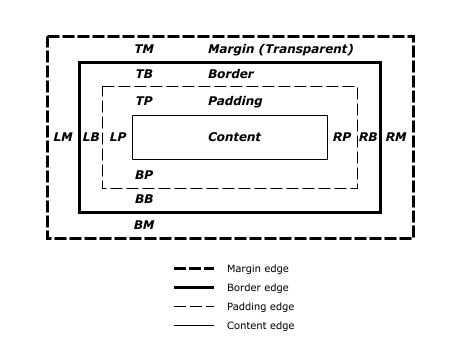
\includegraphics[scale=1]{css/resources/box-mode.png}




\subsubsection{border}

border三个属性 宽度(width), 样式(style), 颜色(color)。 border还有第四个属性radius,但是不影响和模型的定位。

\begin{CSS}[三个粒度]
{border: 2px dashed red;} // 全部3个属性,全部4条边
{border-style: dashed;} // 一个属性,四条边
{broder-left-style: dashed;} // 一个属性,一条边
\end{CSS}

\subsubsection{padding}

内边框

\subsubsection{margin}

外边框。

\begin{CSS}[上 右 下 左]


{margin-top:5px; margin-right:10px; margin-bottom:12px; margin-left:8px;}

{margin: 5px 10px 12px 18px;}

\end{CSS}

如果有值没有写,则取对边的值,如果只写了一个值,则四边都取这个值。


\begin{CSS}[中和外边框和内边框,使不同浏览器效果一致]
* {margin: 0; padding: 0;}
\end{CSS}

\subsubsection{margin 叠加}

(!!!!我记得这和有个什么显示方式有关,默认情况下上下排列才是垂直方向上外边距叠加,需要看文档补充一下)
垂直方向上的外边距会叠加。

外边框叠加,比如有两个段落,第1个段落的下外边距是50px,第2个段落的上外边框为30px,那么他们之间的外边框是50px。因为这种上下外边框相遇的情况下,他们会相互重叠,直到一个外边框碰到另一个元素的边框。



\subsubsection{盒子大小}

对于块级元素,如果没有设置width,那么他的默认值就是auto,结果会让元素的狂度扩充到与父元素同宽;如果添加水平边框,内边距和外边距,会导致内容宽度减少,减少量等于水平边框,内边距和外边距增加之和。

明确设定width之后,块级元素就不会再扩展到与父元素同宽了。盒子width属性指定的只是盒子内容区的宽度,而不是盒子要占住的水平宽度。


\subsection{float \& clear}

\subsubsection{float}

float
\begin{itemize}
\item 值: left, right, none, inhert
\item 初始值: none
\item 继承性: 无
\item 计算值: 
\end{itemize}

替换元素: 

非替换元素:

浮动的一些规则:
\begin{itemize}

\item 会以某种方式将浮动元素从文档流中删除

\item 浮动元素的外边距不会合并

\item 非替换元素浮动,必须指定一个width,否则宽度将为0

\item none表示不浮动

\item 浮动元素的包含块是其最近的块级祖先元素,浮动元素会生成一个块级元素

\end{itemize}


一系列浮动的细节:
\begin{itemize}

\item 浮动元素的左(右)外边界不能超出其包含块的左(右)内边界(这个很明显没啥问题)


\item 浮动元素的左(右)外边界必须是源文档中之前出现的左浮动(右浮动)元素的右(左)边界,除非后出现浮动元素的顶端在先前出现浮动元素的底端下面。


这条规则是用来防止浮动元素相互覆盖的

也就是说,一个元素往左浮动,他必须出现在原来已经左浮动的元素的右边。或者,如果这个浮动元素的顶端在原来浮动元素的下面,那么这个元素就可以一直浮动到父元素的左内边界。

这样就不用放心的浮动元素。

\item 左浮动元素的右边界,不会在其右边右浮动元素的左边界的右边。一个右浮动元素的左边界,不会在其左边的左浮动元素的右边界的左边。

这条规则是用来防止浮动元素重叠的。

\item 一个浮动元素的顶端不能比其父元素的内顶端更高

这个很好理解

\item 如果一个浮动元素在两个合并外边距之间,放置这个浮动元素时,就好像两个元素之间有一个块级父元素。   !!!!!??

这里使用三个段落,浮动中间的段落查看效果


\item 浮动元素的顶端不能比之前所有浮动元素或块级元素的顶端更高。

这个也很好理解,但是记住是浮动元素或者块级元素。这是不是也很好的说明了上面那一条呢?

\item 如果源文档中一个浮动元素之前出现另外一个元素,浮动元素的顶端不能比包含该元素所生成框的任何 ?? 这里少写了吗?

这里说的需要测试,在一个行级元素的内部的元素浮动一下看看。

\item 左(右)浮动元素的左(右)边有一个浮动元素,前者的右(左)边界不能在其包含块的右(左)边界的右(左)边。

这里说的是浮动元素不能够超出包含块的边界,除非他太宽了,本身就放不下。


\item 浮动元素应尽可能高的放。

这个也很好理解。

\item 左浮动元素必须尽可能向左,右浮动元素尽可能向右。

\end{itemize}


clear: left, right, both

clear就是保证元素的左(右)边没有浮动元素。

















